\documentclass[english, 12pt, a4paper, sci, utf8, a-2b, online]{aaltothesis}
%\documentclass[english, 12pt, a4paper, elec, utf8, a-2b, print]{aaltothesis}
%\documentclass[english, 12pt, a4paper, elec, utf8, a-2b, print, twoside]{aaltothesis}

%% FOR USERS OF AMS PACKAGES:
%% * newtxmath used in this template loads amsmath, so
%%   you needn't load it. If you want to use options in amsmath, load it here,
%%   before \setupthesisfonts below to pass the options to amsmath.
%% * If you want to use amsthm, load it here before \setupthesisfonts to avoid
%%   a clash with newtxmath.
%% * If using amsmath with options and you want to use amsthm, load amsthms
%%   after amsmath, as described in the amsthm documentation.
%% * Don't use amsbsym or amsfonts. The symbols [and macros] there are defined in
%%   newtxmath and so clash if used.
%\usepackage[options]{amsmath}
%\usepackage{amsthm}


\setupthesisfonts

\usepackage{graphicx}
\usepackage{longtable}
\usepackage[type={CC}, modifier={by-nc-sa}, version={4.0}]{doclicense}
\usepackage[capitalise]{cleveref}
\usepackage{ifthen}
\usepackage{algorithm}
\usepackage{algpseudocodex}
% \usepackage[usenames,dvipsnames]{color}


\newtheorem{definition}{Definition}
\newtheorem{theorem}{Theorem}
\newtheorem{lemma}{Lemma}
\newtheorem{corollary}{Corollary}
\newtheorem{proposition}{Proposition}

\newcommand{\N}{\mathbb{N}}
\newcommand{\Z}{\mathbb{Z}}
\newcommand{\od}[1][]{\ifthenelse{\isempty{#1}}{\mathrm{OD}}{\mathrm{OD}_{\mathit{#1}}}}
% \newcommand{\od}{\mathrm{OD}} 




\degreeprogram{Mathematics and Operations Research}
\major{Systems and Operations Research}
\univdegree{MSc}
\thesisauthor{Leevi Rönty}

\thesistitle{Graph Neural Network Heuristic for Public Transport Timetable Planning}
%\thesistitle[Title of the thesis]{Title of\\ the thesis}
% \thesissubtitle{A possible subtitle}
%\thesissubtitle[Subtitle of the thesis]{Subtitle of\\ the thesis}

% \place{Otaniemi}
\place{Espoo}
\date{9 February 2023}

\supervisor{Prof.\ Philine Schiewe}
\advisor{Prof.\ Philine Schiewe}

\uselogo{!}

\copyrighttext{\noexpand\textcopyright\ \number\year. This work is
	licensed under a Creative Commons "Attribution-NonCommercial-ShareAlike 4.0
	International" (BY-NC-SA 4.0) license.}{\noindent\textcopyright\ \number
	\year \ \doclicenseThis}


\keywords{concepts that are\spc central to your\spc thesis}
\thesisabstract{
    Abstract placeholder.
}
\begin{document}
\makecoverpage
\makecopyrightpage
\clearpage

\begin{abstractpage}[english]
    \abstracttext{}
\end{abstractpage}


\newpage
\thesistitle{Placeholder title in finnish}
% \thesissubtitle{Opinnäytteen mahdollinen alaotsikko}
\supervisor{Prof.\ Philine Schiewe}
\advisor{Prof.\ Philine Schiewe}
% \degreeprogram{Elektroniikka ja sähkötekniikka}
\date{9.2.2023}
%% The keywords need not be separated by \spc now.
% \keywords{Vastus, resistanssi, lämpötila}
%% Abstract text
\begin{abstractpage}[finnish]
    Abstrakti suomeksi.
\end{abstractpage}


\newpage


\dothesispagenumbering{}


\vspace{5cm}
Otaniemi, 9 February 2023\\

\vspace{5mm}
{\hfill Leevi Rönty \hspace{1cm}}

\newpage
\thesistableofcontents

\cleardoublepage
\section{Introduction}
\label{sec:intro}
% \thispagestyle{empty}
\begin{itemize}
    \item Public transportation affects the lives of many
    \item Low wait times are one component of a good transportation system
    \item One way to affect the transfer wait times is to have schedules that play well together
    \item Bonus: changing the schedule is very cheap, compared to introducing new lines or increasing the frequency of the lines.
    \item Problem: optimal timetable depends on routes used, but routes used depend on the timetable
    \item For optimality, these must be considered at the same time
    \item This is infeasible with the current models
    \item If routes are fixed, it's easier to solve for a good timetable
    \item Objective of the thesis: study how we could predict the optimal routing so that we would be left with the easier-to-solve PESP problem.
    \item Overview of the thesis: we generated data, fitted a GNN on it, evaluated on both generated and given data, checked for generalization, benchmarked etc.
\end{itemize}



% From the passenger's point of view, an efficient public transportation system allows the passengers to travel to their destination quickly. The time spent 

The schedule determines when the vehicles arrive and depart from the stops in a public transport system. From the passenger's point of view, an efficient schedule minimizes the expected travel time. However, optimizing for the travel time is not easy. The optimal schedule depends on the routes the passengers choose to get to their destination, but at the same time the chosen routes depend on the schedule. This means, that to guarantee optimal solutions, we must optimize both the schedule and the passenger routes at the same time. This is much more difficult than optimizing the schedule with a pre-determined passenger routing, as the number of routes that each passenger can choose from can be very large, and in a realistic scenario, we will have a large number of passengers.

In this thesis, we will attempt to develop a heuristic solution method to this integrated optimization problem by trying to predict the optimal routing before solving for the timetable. We will study if a graph neural network model would be able to predict these routes and how the model's predictions would fare against previous heuristics with both small and large public transport networks.

We begin by first reviewing the literature related to the topics of the thesis. We continue by covering the theoretical background for the problem, some simple previous heuristics, and graph neural networks. Then we describe the data generation and the experiments, after which we conclude by presenting the results and analyzing what we learned.

\subsection{Literature review}

% As we are aiming to <> a new GNN heuristic for the TimPass problem, we 

We will study the previous literature from three perspectives. First, we will explore the previous heuristics, solving methods, and formulations related to the TimPass problem as seen in \cite{schmidt2014integrating, schiewe2020periodic}. Next, we review the literature for ML methods in public transport optimization, and lastly, we take a look at ML methods in combinatorial optimization.

The TimPass formulation of \cite{schiewe2020periodic} can be viewed as an extension to the periodic event scheduling problem as described in ???. 


Darwish et al. \cite{darwish2020optimising} used a deep reinforcement learning method to solve the transit network design and frequency setting problem. The obtained results seem promising, yielding state-of-the-art solutions on the Mandl's Benchmark Network. In their formulation, an encoder-decoder network yields a sequence of edges and line start tokens.

Yan et al. \cite{yan2022distributed} applied a multiagent reinforcement learning approach to optimize the timetables for selected bus lines in Beijing. In their approach, the individual passengers and bus drivers are modelled by an agent, that can take real-time information such as weather into account. The proposed solutions yields a 20\% improvement of the operating cost against the real-world timetable.






Three perspectives:
\begin{itemize}
        \item Advances in TimPass tms.?
        \item Previous NN / RL applications in public transport
        \item NN in combinatorial optimization
\end{itemize}

\begin{itemize}
    \item SAT formulations
    \item ???
\end{itemize}

\begin{itemize}
    \item Some RL agents in aperiodic scheduling
    \item 
    \item 
\end{itemize}

\begin{itemize}
    \item "Neural branching and diving" (google)
    \item Some review papers
\end{itemize}

\clearpage
\section{Methods}
\subsection{Event activity network data}


% \begin{definition}[Public transport network]\label{def:ptn}
%     A public transport network (PTN) is a graph with a set of stops $V$ connected by a set of direct connections between the stops $E$. We consider the edges to be undirected.
% \end{definition}


% In \cref{def:ptn} we showed xyz.

% prujaa: ???



Before we can define event activity networks, we have to define a few other things. A \textit{public transport network} (PTN) is a simple graph PTN = $(S, R)$ with a set of stops $S$ and a set of direct connections between the stops $R$. A PTN describes the underlying transportation infrastructure of a public transport system. Note, that in this case, we don't differentiate between transportation modes like busses and trains. In general, a real public transportation system would have multiple modes of transportation, but we ignore this for now, as the developed heuristic could be easily extended to a multimodal case. We also consider the connections to be undirected. This only makes the modelling a bit easier, but one could also have a PTN with directed edges. The PTN could also be non-simple, but that notation would make a difference only if there were either capacity constraints per connection or if multiple modalities were used.

We are interested in the periodic instead of the aperiodic scheduling problem. In the periodic setting, we have a \textit{period} $T \in \N$ which defines the time interval at which various events and activities are repeated. This period could be for example 60 minutes, one day, or something else. The appropriate period length depends on what kind of schedule we aim to optimise. Note that in general, the period could be a positive real number, but we consider it to be an integer to follow the convention established in \cite{schiewe2020periodic}.


% TODO: miten merkataan simple path tässä tapauksessa? Onko siis ordered setti / lista stoppeja?
A \textit{line} $l$ is a simple path in a PTN. A \textit{line concept} is a set of lines $L$ with associated frequencies $f_l \in \N$ for all $l \in L$. A frequency determines how often a line is served within the period $T$. We assume the lines to be bidirectional, meaning that the vehicles travel the line in both directions.

From the line concept, we can construct the event activity network (EAN). The graph EAN = $(E, A)$ has a set of events $E$ and a set of activities $A$ connecting the events. For the events, we have two types of them: $E = E_\text{arrival} \cup E_\text{departure}$. As the names suggest, the disjoint sets $E_\text{arrival}$ and $E_\text{departure}$ contain the events describing vehicle arrivals and departures from the stops. To simplify the notation, we define the set of available repetition numbers $R_l = \{1, \dots, f_l\}$ and the set of available directions $D = \{\text{fw}, \text{bw}\}$. More formally, the sets are defined as follows:
\begin{align*}
    E_\text{arrival} &= \{
        (\text{arr}, s, l, d, r) : l \in L, s \in l, d \in D, r \in R_l
    \} \\
    E_\text{departure} &= \{
        (\text{dep}, s, l, d, r) : l \in L, s \in l, d \in D, r \in R_l
    \}
\end{align*}
As seen in the definition, the events consist of the event type, the stop, the line, the driving direction (either forward or backward), and the line repetition number which is used to differentiate between separate repetitions of the line in the periodic case.

For the activities, we also have multiple distinct types: drive, wait, change, and sync. Thus, we have that $A = A_\text{drive} \cup A_\text{wait} \cup A_\text{change} \cup A_\text{sync}$. The formal definitions are as follows:
\begin{align*}
    A_\text{drive} =& \{(
        (\text{dep}, s_1, l, \text{fw}, r),
        (\text{arr}, s_2, l, \text{fw}, r)
    ): l \in L, (s_1, s_2) \in l, r \in R_l\} \cup \\
    &\{(
        (\text{dep}, s_2, l, \text{bw}, r),
        (\text{arr}, s_1, l, \text{bw}, r)
    ): l \in L, (s_1, s_2) \in l, r \in R_l\} \\
    A_\text{wait} =& \{(
        (\text{arr}, s, l, d, r),
        (\text{dep}, s, l, d, r)
    ): l \in L, s \in l, d \in D, r \in R_l\} \\
    A_\text{change} =& \{(
        (\text{arr}, s, l_1, d_1, r_1),
        (\text{dep}, s, l_2, d_2, r_2)
    ): \\&l_1 \in L, l_2 \in L, l_1 \neq l_2, s \in l_1 \cap l_2, d_1 \in D, d_2 \in D, r_1 \in R_{l_1}, r_2 \in R_{l_2}\} \\
    A_\text{sync} =& \{(
       (t, s, l, d, r-1),
       (t, s, l, d, r)
    ):\\ &t\in \{\text{arr}, \text{dep}\}, l \in L, s \in l, d \in D, r \in R_l, r \geq 2 \}
\end{align*}

In plain English, the drive activities correspond to the driving activity between stops. The activities connect the line's departure events to the corresponding arrival events. The wait activities correspond to the vehicle staying at the station, waiting to e.g. load and unload passengers. The wait activities connect arrival events to departure events. The drive and wait activities are demonstrated in \cref{fig:drive-wait-demo}. The change activities denote the line transfers that the passengers may take. The activities link the arrivals to departures within the same stop that do not belong to the same line. The idea of change activities and multiple lines at the same stop is shown in \cref{fig:change-demo}. The sync activities are a bit different from the other activities, as the passengers can't travel along those edges. For this reason, we note the set of activities usable for passenger routing as $A_\text{routable} = A \setminus A_\text{sync}$. The only use for sync activities is for defining constraints on the timetable to have some predefined spacing among the repetitions of the lines. How sync activities are connected is shown in \cref{fig:sync-demo}. Defining the constraints on all sync activities is not mandatory. In that case, the sync activities without constraints are essentially pointless.


\begin{figure}
    \centering
    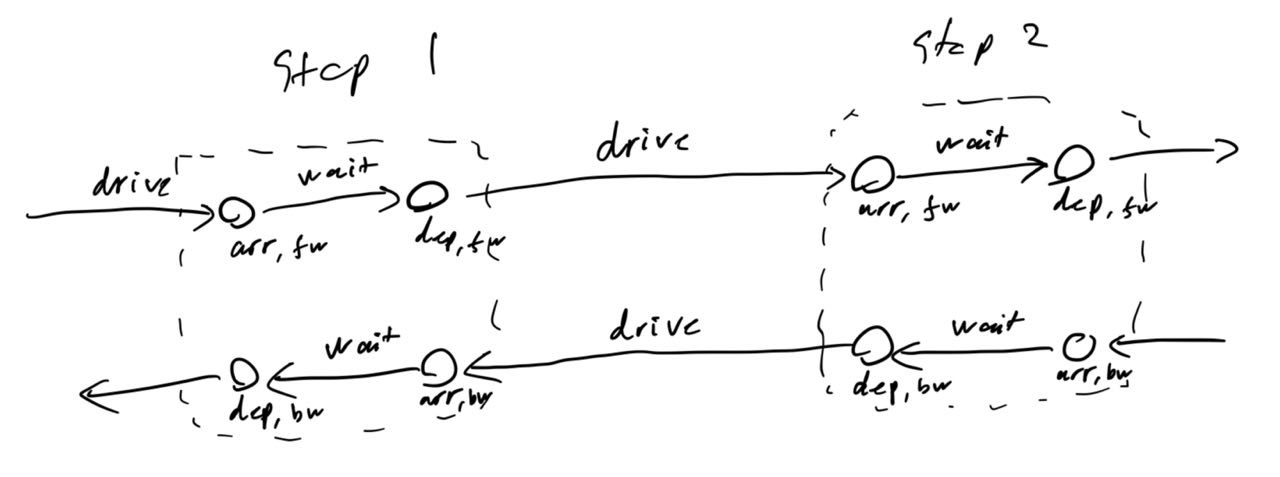
\includegraphics[width=1.0\textwidth]{figures/drive-wait-demo.jpg}
    \caption{Demonstration for arrival and departure events, drive and wait activities, and line directions.}
    \label{fig:drive-wait-demo}
\end{figure}

\begin{figure}
    \centering
    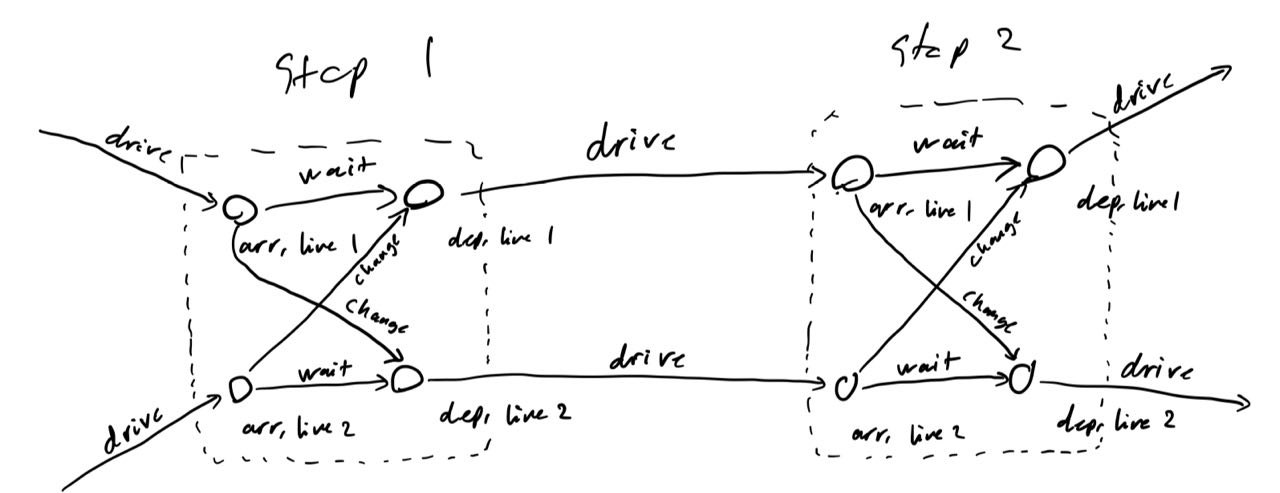
\includegraphics[width=1.0\textwidth]{figures/change-demo.jpg}
    \caption{Demonstration for multiple lines at a stop and change activities.}
    \label{fig:change-demo}
\end{figure}

\begin{figure}
    \centering
    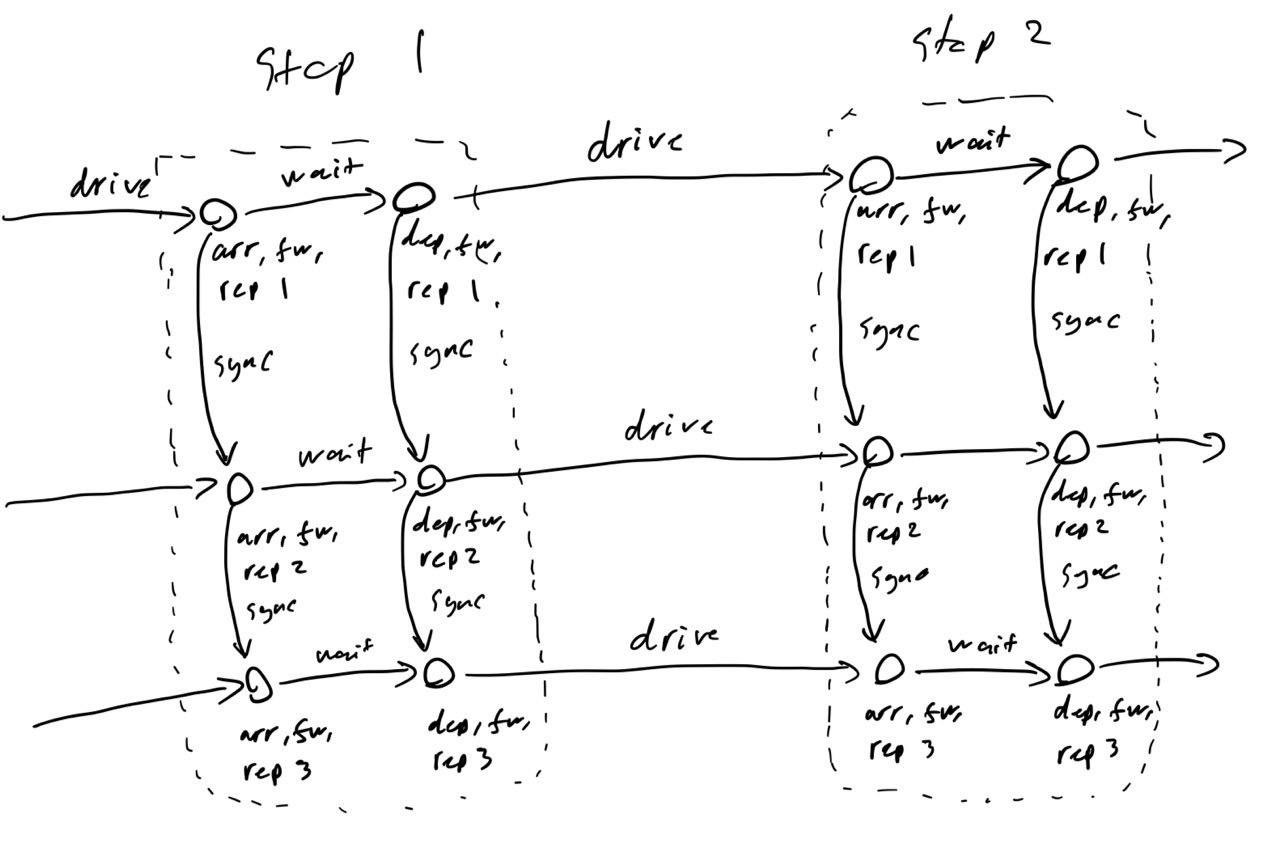
\includegraphics[width=1.0\textwidth]{figures/sync-demo.jpg}
    \caption{Demonstration for higher frequency lines and sync activities.}
    \label{fig:sync-demo}
\end{figure}

% joku PTN-kuvaus, pari esimerkkilinjaa
% käppyröitä, joilla havainnollistetaan miltä eanit näyttää

% MIP-ongelmien osuuteen:
    % ODs
    % schedule
    % bounds & penalties on events


% We model the public transport system to have a set of stops, and some demand between those stops. The demand represents the number of passengers wishing to travel from a given node to another node. The demand is directed, i.e. we allow the demand to be different from stop $a$ to stop $b$ than from $b$ to $a$.  % TODO: tähän joku matemaattinen notaatio, millä demandia merkataan??

% Before diving deeper into the networks, we must recognize the two types of event activity networks: periodic and aperiodic. In the periodic setting, we assume the timetable to repeat periodically, e.g. every 60 minutes. Aperiodic timetable does not assume this repetition, making it suitable for modelling instances with varying line frequencies. For example, the interval between departures could be shorter during the rush hour than in the middle of the night.

% In this study, we consider only the periodic case. Firstly, for the aperiodic formulation to be useful, we would also need time-dependent demand between stops. Realistic data for this is harder to come by. Secondly, we are still testing if this heuristic method is even feasible. Testing the approach on periodic problems is fine, as extending it to the aperiodic case should be simple.

% Event activity networks are directed graphs that consist of nodes called events and the edges connecting the events called activities. This structure is used to model how passengers travel in the transportation system on an individual vehicle level.

% The network has two types of nodes: arrivals and departures. On top of node type, each event has the following attributes: stop id, line id, line direction, and in the case of periodic EANs, the repetition number. These attributes are enough to uniquely identify all nodes.

% The activities connecting events 


% \begin{itemize}
%     \item Describe the difference between periodic and aperiodic, briefly justify focusing only on the periodic case. 
%     \item OD pairs: how many customers wish to travel from one stop to another. In general could be time-dependent, but easier if it's not.
% \item Specification for an EAN with plenty of graphs: node types and features, edge types and features, how these are combined to describe a public transportation system.
% \item Change penalty and the perceived travel time, related to the edge features.
% \item Note about capacity limits: in general we could have bounds on the passenger count, but the problem is much easier without this.
% \item Graphs:
% \item One line going through few stops, both ways. Points to demonstrate: how one line is described with the EAN
% \item Two lines on a stop, omit the reverse direction of the lines to keep the graph a bit clearer, freq > 1 for one line. Points to demonstrate: How transfers, headways, and sync edges are used.
% \end{itemize}

\subsection{Integer programming problems}

We can define a schedule for the events in an EAN. The event times are noted as $\pi_e \in \{0, \dots, T-1\}$ for all events $e \in E$. As we are working with a periodic schedule, all the event occurrence times must be lower than the period of the schedule $T$. As noted previously, we could have a real-valued schedule instead of a discrete one, but once again we follow the previous formulation.

The activities in the EAN are used to define constraints on the upper and lower bounds for activity durations. For all activities $a \in A^0$, we have the lower bound $L_a \in \N$ and upper bound $U_a \in \N$. For the bounds, we of course must also have that $0 \leq L_a \leq U_a$. The activity duration for activity $a = (i, j)$ itself is calculated as follows: $\text{duration} = L_a + (\pi_j - \pi_i - L_a)\ \text{mod}\ T$. The lower bound term outside of the modulo ensures, that the lower bound is respected. The term inside the modulo is the "slack" time we have due to the schedule not aligning perfectly with the lower bound. As formulated, the duration is guaranteed to be greater or equal to the lower bound. For the given timetable $\pi$ to be feasible, for all activities $a \in A$ we must have that the upper bound holds: $L_a + (\pi_j - \pi_i - L_a)\ \text{mod}\ T \leq U_a$.

As the modulo does not fit well into linear programming, we replace the modulo term with a multiplier $z_a \in \Z$ times $T$: $\text{duration} = L_a + \pi_j - \pi_i - L_a z_aT$. As the multiplier $z_a$ can be chosen freely, this is equivalent to the formulation with the modulo.


Along the EAN, we need information on the passenger demand between the stops of the PTN. We note the number of passengers wanting to travel from stop $i$ to stop $j$ as $\od_{i,j} \in \N$. Not all stop pairs have demand: we express the set of stop pairs with non-zero demand as $\od = \{(i,j): i \in S, j \in S, \od_{i,j} > 0\}$.

For routing of the passengers, we assume a fixed routing that is given beforehand. When routing the passengers, each OD pair assumes some path from $i$ to $j$ through the EAN, and for the chosen path edges the weight $w_a$ is incremented by the number of passengers using that route. We will later return to routing in a subsequent section. For now, it's enough to recognize, that we have a weight $w_a \in \N$ for all routable activities of the EAN.

Now we can express the PESP problem. Instead of minimising the real total travel time $\sum_{a \in A_\text{routable}} w_a (\text{duration}_a)$, we minimise the total perceived travel time. In perceived travel time, we add the "perceived penalty" duration to the real duration. In principle, the penalty $\text{penalty}_a$ could be any real value, but we consider it as a penalty for transferring between lines, i.e. a penalty that is non-zero only for change activities and for those activities the penalty is some positive integer.

% From the OD demand, we use some routing scheme to obtain weights.  % TODO: more formally, good points in prev. literature.

Cite this: \cite{schiewe2020periodic}.

\begin{align}
    \textrm{min.} \quad  &\sum_{a \in A_\text{routable}} w_{a} (\pi_j-\pi_i+z_aT + \text{penalty}_a) \\
    \textrm{s.t.} \quad &L_a \leq \pi_j-\pi_i+z_aT  \leq U_a \quad a =(i,j)\in A_0 \\
    &\pi_i \in \{0, \dots, T-1\} \quad i \in E_0\\
    &z_a \in \Z \quad a \in A_0
\end{align}

The formulation for the PESP problem using the schedule $\pi$ is correct, but it's not the most efficient one available. Instead of explicitly defining the times for the events, we could instead define just the activity durations directly. We note the activity duration as $x_a \in \N$. Now the constraint on activity durations is much simpler: $L_a \leq x_a \leq U_a\ \forall a \in A$. This formulation also reduced the number of symmetrical solutions: when defining the event times explicitly, we could always transform a feasible timetable into another by rotating the event times through the period $T$.
% TODO: any research on why the cycle-basis is more efficient?

However, now we need to take the cycles in the EAN into account. In \cref{fig:cycle-example}, we have the activities a, b, c, d, e, and f. For the activity durations to be consistent, we must have that the difference of duration of the upper path $x_a + x_b + x_c$ and lower path $x_f + x_e + x_d$ must be an integer multiple of the period $T$. More formally, $x_a + x_b + x_c - x_d - x_e - x_f = zT$ for some $z\in \Z$. The difference can be a multiple of the period as we are dealing with a periodic timetable, otherwise the difference should be zero.

\begin{figure}
    \centering
    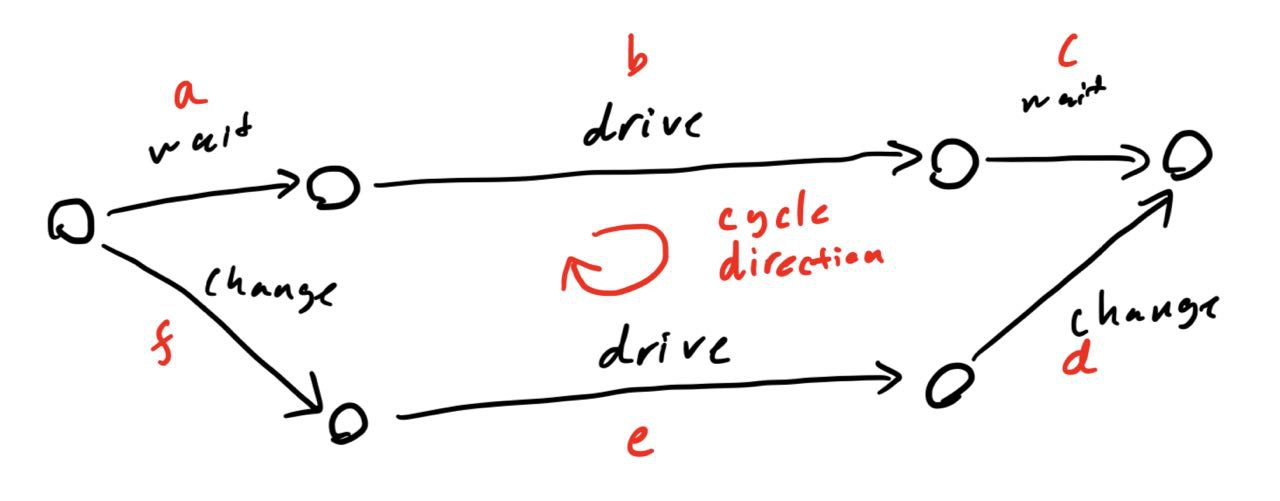
\includegraphics[width=\textwidth]{figures/cycle-basis-demo.jpg}
    \caption{Cycle consistency example.}
    \label{fig:cycle-example}
\end{figure}

In the cycle basis formulation, we consider cycles regardless of the edge direction, but the cycle does have a direction. All the edges of a cycle $c$ belong either to the set of "positive edges" $c_+$ or the set of "negative edges" $c_-$, based on the direction of the edges along the cycle. In the example of \cref{fig:cycle-example}, we would have that $c_+ = \{a, b, c\}$ and $c_- = \{d, e, f\}$. In more general terms, for a cycle $c$ to be consistent, we must have
\begin{align}
    \sum_{a\in c_+}x_a - \sum_{a \in c_-}x_a = zT\ \exists z \in Z.
\end{align}

A EAN may have many cycles, but luckily we don't have to check the condition for all cycles. We can construct a cycle basis for the EAN and checking the condition for that basis is enough. We denote the cycle basis as $C$.  % TODO: proof / cite a source showing that cycle basis is enough to check. Maybe some words on how the cycle basis is constructed?


Now we may define the cycle basis formulation for the PESP problem. The formulation is quite similar to the original definition, but now the activity duration is expressed in a very concise way and we have the additional cycle consistency constraint:
\begin{align}
    \textrm{min.} \quad  \sum_{a \in A_\text{routable}} w_{a} (x_a + \textrm{penalty}_a) \\
    \textrm{s.t.} \quad  \sum_{a\in c^+} x_a - \sum_{a\in c^-} x_a & = z_c T \quad c \in C \\
    L_a \leq x_a & \leq U_a \quad a \in A \\
    z_c &\in \Z \quad c \in C \\
    x_a &\in \Z \quad a \in A
\end{align}

In the TimPass problem, we are free to choose the route used for each OD pair as we minimise the total perceived travel time. However, to represent the routes from stop $i$ to stop $j$, we would prefer to have all the possible paths start and end to the same nodes. To achieve this, we introduce the auxiliary events $E_\text{aux}$ and auxiliary activities $A_\text{aux}$. For the auxiliary events, we have one origin and departure event for each stop: $E_\text{aux} = \{(t, v) : t \in \{\text{origin}, \text{destination}\}, v \in V\}$. For the auxiliary activities, we have an edge from all auxiliary origin events to the corresponding stop's events and an edge from all stop's events to the corresponding destination auxiliary event:
\begin{align}
    A_\text{aux} = \{&((\text{origin}, s_1), e): s_1 \in V, e = (t, s_2, l, d, r) \in E, s_1 = s_2\} \cup \\
    \{&(e, (\text{destination}, s_1)): s_1 \in V, e = (t, s_2, l, d, r) \in E, s_1 = s_2\}
\end{align}

To note if the activity $a$ is part of the chosen path between stops $u$ and $v$, we have the variable $p_a^{uv} \in \{0, 1\}$. This allows us to set up some constraints on what is considered a valid path. For a from stop $u$ to stop $v$ to be valid, it must start at the event $(\text{origin}, u)$ and end at $(\text{destination}, v)$. Additionally, the path must be connected from the origin all the way to the destination, i.e. for all events that are not auxiliary events we must have an equal number of active edges leading to it and out of it. 

We can formalise this by introducing a node-arc-incidence matrix $M$ and an origin-destination vector $b =(b_e)_{e\in E \cup E_\text{aux}}$. For a origin-destination pair $(u, v) \in \od$, the origin-destination vector elements are:
\begin{align}
    b_e = \begin{cases}
        -1\ \text{if}\ e=(\text{origin}, u)\\
        +1\ \text{if}\ e=(\text{destination}, v)\\
        0\ \text{otherwise}
    \end{cases}
\end{align}

For the node-arc incidence matrix $M=(m_{e, a})_{(e, a) \in (E \cup E_\text{aux}) \times (A \cup A_\text{aux})}$, we have that the element is minus one if the activity leads away from the event, one if the activity leads to the event and zero otherwise. Formally:
\begin{align}
    m_{e, a} = \begin{cases}
        -1\ \text{if}\ a = (e, t)\ \exists t \in E \cup E_\text{aux}\\
        1\ \text{if}\ a = (t , e)\ \exists t \in E \cup E_\text{aux}\\
        0\ \text{otherwise}
    \end{cases}
\end{align}

Armed with this notation, we can finally construct the constraint necessary for the set of active flow variables to constitute a valid path from stop $u$ to stop $v$:
\begin{align}
    M \cdot (p_a^{uv}) = b \quad \forall uv \in \od
\end{align}
This constraint does not actually prevent the flow variables from creating a cycle, but as we are minimising the total perceived travel time, those cycles would be non-optimal and thus they will not occur in optimal solutions.

We can express the total perceived travel time as the sum of perceived travel times over all OD pairs. Thus, we are minimising the following expression:
\begin{align}
    \sum_{uv \in \od}\od_{uv} \sum_{a \in A_\text{routable}}p_a^{uv}(x_a + \text{penalty}_a)
\end{align}
However, we have a problem as we hope to get a linear integer programming problem. Now we have $p_a^{uv}x_a$, which is not linear as both terms are decision variables. Luckily, as the flow variable $p_a^uv$ can only be either 0 or 1, we can linearise this expression quite easily.

We create the linearization decision variable $lin_a^{uv}$ for all $a \in A$ and $uv \in \od$. We aim to always have $lin_a^{uv} = p_a^{uv}(x_a + \text{penalty}_a)$ without explicitly stating this equality, as the right hand side has the non-linear term. We achieve this by constructing suitable constraints for the linearization term.

Let $B$ be some large integer for which $B \geq x_a + \text{penalty}_a\ \forall a \in A$. With this value, we can come up with the following set of constraints:
\begin{align}
    &lin_a^{uv} \geq 0 \\
    &lin_a^{uv} \leq p_a^{uv} B \\
    &lin_a^{uv} \leq x_a + \text{penalty}_a \\
    &lin_a^{uv} \geq x_a + \text{penalty}_a - (1 - p_a^{uv}) B
\end{align}
Now, if $p_a^{uv} = 0$, we must have that $lin_a^{uv} = 0$. If $p_a^{uv} = 1$, then $lin_a^{uv} = x_a + \text{penalty}_a$.

Now we can finally express the TimPass problem with the cycle basis formulation. We omit the linearization term and constraints for clarity, but in practice, the linearization must be done for commonly available solvers to function properly.
\begin{align}
    \textrm{min.} \quad  \sum_{\mathit{uv} \in \textrm{OD}} \od_{\mathit{uv}} \sum_{a \in A_\text{routable}} p_{a}^{\mathit{uv}} (x_a + \textrm{penalty}_a) \\
    % \textrm{min.} \quad  \sum_{\mathit{uv} \in \textrm{OD}} \od_{\mathit{uv}} \sum_{a \in A_\text{routable}} lin_a^{uv}) \\
    \textrm{s.t.} \quad  \sum_{a\in c^+} x_a - \sum_{a\in c^-} x_a & = z_c T \quad c \in C \\
    L_a \leq x_a &\leq U_a \quad a \in A \\
    % x_a &\leq U_a \\
    M (p_{a}^{\mathit{uv}})_{a\in A} &= b^{\mathit{uv}} \quad \mathit{uv} \in \textrm{OD}\\
    x_a &\in \Z \quad a \in A \\
    z_c &\in \Z \quad c \in C \\
    p_a^{\mathit{uv}} &\in \{0, 1\} \quad a \in A, \mathit{uv} \in \textrm{OD}
\end{align}

% TODO: preprocessing??
\begin{itemize}
    % \item Introduce auxiliary events used in the TimPass formulation.
    % \item Introduce how the routing constraint matrix $A$ and vector $b$ are defined.
    % \item Briefly describe how the linearization trick for the objective works.
    \item Describe how preprocessing works to reduce the number of routes we have to consider.
    \item Describe how multiple solutions are obtained by turning the optimal objective into a constraint and generating a new objective with random weights on the routing variables. Maybe we can cite Helmi's work here?
\end{itemize}
\textbf{TODO: the formulation below does not take sync activities into account. Fix by including e.g. $p_{\text{some sync index}} = 0$.}
\textbf{TODO: Include preprocessing constraint.}

The given formulation for the TimPass problem works, but we are left with many flow variables. Luckily, there is a way to reduce the complexity by calculating which flows can never exist in the optimal solution. This method is first presented in \cite{schiewe2020periodic}. 

We define the function $SP_{u,v}(D)$ to be the function, that given the set of durations $D$ for the activities, calculates the shortest path between nodes $u$ and $v$ in the given EAN. This shortest path can be calculated with e.g. Dijkstra's algorithm. We can calculate the length of the path with the function $len(p, D)$, which calculates the length of the path $p$ with the durations $D$. We define $len(p, D) = \sum_{a \in p} D_a$.

We can use the upper and lower bounds for the durations in the functions defined above. However, as in the TimPass problem we are dealing with perceived travel times, we should include the penalty term in the duration. Thus, let us define $L^+ = \{L_a + \text{penalty}_a:a\in A\}$ and $U^+ = \{U_a + \text{penalty}_a:a \in A\}$. Now we can use these to calculate which flow variables $p_a^{uv}$ can never be active in the optimal solution.

In \cref{alg:preprocessing} we present the algorithm for calculating which flow variables can be safely set to zero.

% TODO: does this even make sense to represent this way? Definitions in a for loop may not be the most interesting thing.
{
    \color{red}
    \textbf{TODO:} \textit{Does expressing the preprocessing in this way even make sense? ofc. this is how it's calculated, but the definition does not benefit from the for-loops.}
}
\begin{algorithm}
    \caption{Flow variable preprocessing}
    \label{alg:preprocessing}
    \begin{algorithmic}
        \State Initialise $P \gets \emptyset$
        \State Calculate $\beta := len(SP_{u,v}(U^+), U^+)$
        \Comment{Longest possible route length from $u$ to $v$.}
        \For{$e \in E$}
            \State Calculate $\gamma_e := len(SP_{u,e}(L^+), L^+)$
            \Comment{Shortest possible path length from $u$ to $e$}
            \State Calculate $\delta_e := len(SP_{e,v}(L^+), L^+)$
            \Comment{Shortest possible path length from $e$ to $v$}
        \EndFor
        \For{$a = (i, j) \in A$}
            \If{$\gamma_i + L_a + \delta_j > \beta$}
                \State $P \gets P \cup \{a\}$
                \Comment{The activity can never belong to the shortest path with any timetable, so we ignore it.}
            \EndIf
        \EndFor
    \end{algorithmic}
\end{algorithm}
    
\subsection{Shortest path routing heuristic}

\begin{itemize}
    \item Idea: use lower bounds + penalties as the edge duration, use Dijkstra's alg to calculate the shortest paths between each OD pair -> accumulate demand for OD pair to be a weight / demand for each activity along the shortest path.
    \item Use obtained weights in PESP
    \item Note about routing: we assume, that the passengers are happy to leave at any time during the period. We are minimizing just the time passengers spend going from origin stop to destination stop.
    \item Note about capacity restrictions: as we don't have any, routing everyone through the same route is fine.
\end{itemize}

\subsection{GNNs}
\begin{itemize}
    \item Neural networks in general: lots of additions and multiplications, with some non-linear layers
    \item How message passing works in general: node embedding to message, send msg to neighbouring nodes, aggregate msgs in some order-invariant way (e.g. attention, sum, max, mean), update node embedding
    \item Can be repeated multiple times -> node embeddings
    \item Node embeddings can be used for downstream tasks
    \item Trained with backpropagation of loss gradient
\end{itemize}


\subsubsection{Positional encodings}
\begin{itemize}
    \item Used laplacian eigenvector positional encodings
    \item Describe why PEs are often used to enable GNNs to distinguish different structures
    \item Briefly describe how this PE method works
    \item Briefly discuss other alternatives for PE choices
\end{itemize}

\subsubsection{Network architecture}
\begin{itemize}
    \item Using HGT for generating node embeddings, MLP for turning node embeddings to predictions.
    \item Injecting PEs to the problem instances before HGT
    \item Describe how hgt generates messages w/ relation information and how message aggregation with attention works.
    \item Justify the choice of architecture: can use information about relation type, good benchmark results
    \item Include a diagram describing the architecture
\end{itemize}


\subsection{Heuristic evaluation method}
\begin{itemize}
    \item For heuristics that assign weights to activities, that are then used to solve PESP
    \item Process in short: solve pesp, use obtained time table to generate shortest path routing, calculate the real objective value from shortest paths and obtained event durations.
    \item Reasoning for doing all this: the weights obtained from the GNN may be scaled arbitrarily (just a prediction, not necessarily unbiased / ) -> we must rescale the weights so that the weights represent 
\end{itemize}

\clearpage
\section{Experiment setup}
\subsection{Data generation}

To train the neural network, we generated a large number of EANs for which we could solve the TimPass problem. All problems use the same available PTN with varying lines, frequencies, and demands. We use a period of 60.

First, we listed all available lines with at least three stops. Then, we sampled the number of lines uniformly between two and four. If the set of lines would be disconnected we would resample the lines to get connected stops.

After the set of lines was determined, we would sample the line frequencies between one and four. We would weight lower frequencies more if the number of previously sampled lines was large. This ensures, that on average the problems are roughly equally as easy to solve.

For the lines with a frequency greater than one, we generate sync activities between all events in sequential line repetitions. By setting the sync upper and lower bounds to be equal to the period divided by the line frequency, we ensure even spacing of the departures.

Once we have all the edges in the EAN, we can sample the upper and lower bounds. We sample the bounds for lines and stop pairs, meaning that the activities belonging to the same line with the same stops as endpoints have the same bounds. We also sample the transfer edge penalties.


Once we have the lines and frequencies, we can sample the demands between stops present in the EAN. 


\begin{itemize}
    \item Base ptn on top of which lines are generated (include graph)
    \item Generation process goes roughly like this:
    \item Enumerated all lines with at least three stops
    \item Sampled random lines and line frequencies, with a weight on frequencies to reduce the probability of instances being very large
    \item Randomized drive durations
    \item Generate random demands for all OD pairs
\end{itemize}

\subsection{Data representation as a heterogenous graph}
\begin{itemize}
    \item Describe how heterogenous graphs are represented in torch\_geometric -> some data conversions are needed
    \item Edge features not included in the architecture -> we turn edges with features to nodes, connecting them with special edges to the original edge endpoints
    \item Remove stop and line ids from features, describe how stops and lines are represented as only the identity of the id is important, not the ordering of the ids.
    \item Additional feature: shortest path weights
    \item Type one-hot encodings
    \item Normalizations for values, easier for neural networks to learn this way
    \item OD demand representation
    \item Included metapaths, as otherwise edge feature nodes could suffer from the lack of connections.
\end{itemize}


\subsection{Training}
\begin{itemize}
    \item Describe hyperparameters and hyperparameter optimization with Bayesian search
    \item Trained on triton with xyz hardware
\end{itemize}
\clearpage
\section{Results}
\begin{itemize}
    \item Should hyperparameter optimization results be listed here or put in an appendix? Maybe not very relevant for the thesis apart from the number of layers and how that relates to long-range dependencies.
\end{itemize}
\subsection{Heuristic performance}

\begin{itemize}
    \item We compared heuristic performances on generated evaluation problems and some problems from Timpasslib
    \item Table: mean, median, and std of optimality gap and loss for both heuristics on the generated problem instances
    \item Scatter plot of GNN gap vs SPR gap
    \item (Scatter plot of GNN loss vs SPR loss, would this be useful?)
    \item Calculate how often GNN beats SPR
    \item Calculate how often we get optimal solutions
\end{itemize}

\subsection{Relation of loss and heuristic optimality gap}

\begin{itemize}
    \item GNN heuristic has an inbuilt assumption that the optimality gap gets smaller as loss decreases
    \item True when loss is very small, otherwise correlation is low
    \item Plot of gap vs loss with both GNN and shortest path routing, points colored by heuristic
\end{itemize}


\subsection{Theoretical lower bound without preference of solutions}
\begin{itemize}
    \item Multiple solutions to TimPass exist, we pick the "right" one essentially at random
    \item We are using mse loss -> the loss would be minimized when we predict the expected value of the optimal solution
    \item Multiple solutions -> we are actually not predicting an optimal solution, but something else
    \item Empirically, the lower bound for the loss would be the variance of the obtained weights
    \item Got an estimate of 0.00199 -> we couldn't get a loss lower than that with this dataset without the preference order.
\end{itemize}


\clearpage
\section{Discussion}
\begin{itemize}
    \item Overview of the results: no consistent improvement, 
    \item Discuss limitations of GNNs: e.g. information squashing, long range dependencies (many benchmarks for tasks with short-range dependencies), other points discussed in the papers related to gnn limitations
    \item Any potential new ideas to make GNNs work in this problem setting?
\end{itemize} 

\clearpage
\section{Summary}
\label{sec:summary}

\clearpage
\thesisbibliography

\bibliographystyle{IEEEtran} 
% \bibliographystyle{apalike} 
\bibliography{refs}


\clearpage
\thesisappendix

\end{document}
